\documentclass[aspectratio=169, 10pt]{beamer}

% Academic Minimalist Theme: Pure Work, Zero Visual Distraction
\usetheme{default}
\usecolortheme{dove}

% Typography & Packages
\usepackage{amsmath, amssymb, amsfonts}
\usepackage{booktabs}
\usepackage{graphicx}
\graphicspath{{../figures/}{./figures/}{../}{./}}
\usepackage{tabularx}
\usepackage{caption}
\usepackage{colortbl}
\usepackage{tikz}
\usetikzlibrary{positioning, arrows.meta}

% Slide Formatting
\setbeamertemplate{navigation symbols}{}
\setbeamertemplate{footline}[frame number]
\setbeamertemplate{frametitle}{\vspace{0.2cm}\textbf{\insertframetitle}\par\vspace{0.06cm}\hrule\vspace{0.12cm}}
\setbeamerfont{frametitle}{size=\large, series=\bfseries}
\setbeamerfont{title}{size=\LARGE, series=\bfseries}

% Clean Academic List Typography
\setbeamertemplate{itemize item}{\raisebox{0.15ex}{\scalebox{0.65}{$\bullet$}}}
\setbeamertemplate{itemize subitem}{\textendash}
\setbeamertemplate{enumerate item}{\small\textbf{\insertenumlabel.}}

\begin{document}

% =============================================================================
% SLIDE 1: Title & Strategic Overview
% =============================================================================
\begin{frame}
  \centering
  \vspace{0.7cm}
  {\LARGE \textbf{Implementation and Sensitivity Optimization of Low-Bit AWQ}}\par
  \vspace{0.2cm}
  {\large \textbf{for On-Device Edge LLM Inference on Unified Memory}}\par
  \vspace{0.3cm}
  \rule{0.5\linewidth}{0.6pt}\par
  \vspace{0.3cm}
  {\normalsize \textbf{Neeraj Kumar} (\texttt{20262603008}) \quad $\cdot$ \quad \textbf{Ashish Dwivedi} (\texttt{20262603003})}\par
  \vspace{0.12cm}
  {\footnotesize Department of Artificial Intelligence \\ Indian Institute of Information Technology Vadodara - ICD}\par
  \vspace{0.35cm}
  {\scriptsize \textbf{AI Lab Course Project Evaluation \& Base Paper Dissection} \quad $\cdot$ \quad November 2026}
\end{frame}

% =============================================================================
% SLIDE 2: Problem Statement & Memory Wall Derivation
% =============================================================================
\begin{frame}{1. The Core Bottleneck: Memory Bandwidth in LLM Decoding}
  \vspace{-0.2cm}
  \begin{columns}[T]
    \begin{column}{0.48\textwidth}
      \footnotesize
      \textbf{Autoregressive Generation ($\text{Batch}=1$):}
      \begin{itemize}
        \item Sequential token generation ($y = W x$).
        \item For every single token, all model weights ($P$ parameters) must be read from off-chip DRAM.
      \end{itemize}

      \vspace{0.08cm}
      \textbf{Derivation of Arithmetic Intensity ($\mathcal{I}$):}
      \[
        \mathcal{I} = \frac{\text{Work (FLOPs)}}{\text{DRAM Bytes}} = \frac{2P\text{ FLOPs}}{2P\text{ Bytes}} = \mathbf{1.0\text{ FLOP/B}}
      \]
      \begin{itemize}
        \item \textbf{Apple M1 Knee:} $\frac{5.2\text{ TFLOPS}}{68.25\text{ GB/s}} = \mathbf{76.5\text{ FLOP/Byte}}$.
        \item System is $100\%$ memory-bound; cores sit $>90\%$ idle!
        \item \textbf{W4A16 Quantization:} Shrinks weights by $4\times$, boosting intensity to $\mathbf{4.0\text{ FLOP/B}}$ ($4\times$ throughput speedup).
      \end{itemize}
    \end{column}

    \begin{column}{0.52\textwidth}
      \centering
      \vspace{0.05cm}
      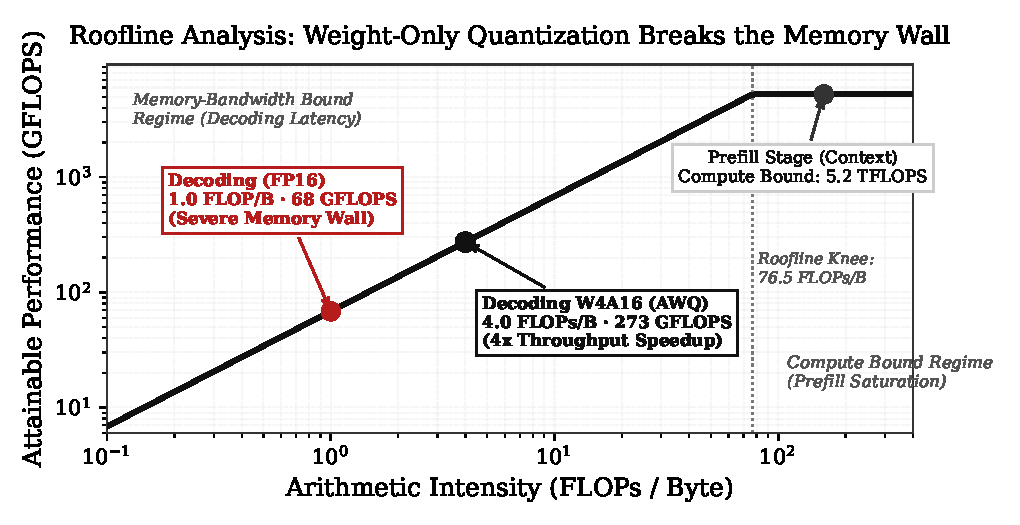
\includegraphics[width=0.92\linewidth]{roofline_memory_wall.pdf}
      \vspace{-0.15cm}
      {\scriptsize \textbf{Figure:} Roofline model on Apple M1. W4A16 shifts arithmetic intensity by $4\times$, breaking the memory wall.}
    \end{column}
  \end{columns}
\end{frame}

% =============================================================================
% SLIDE 3: Prior Art & The Saliency Paradox
% =============================================================================
\begin{frame}{2. Prior Art Failure \& The Saliency Paradox}
  \vspace{-0.2cm}
  \begin{columns}[T]
    \begin{column}{0.50\textwidth}
      \footnotesize
      \textbf{Why Prior Quantization Fails on Edge:}
      \begin{itemize}
        \setlength{\itemsep}{0.08em}
        \item \textbf{QAT:} Retraining is intractable ($>100\times$ pretraining compute).
        \item \textbf{Naive RTN:} Rounds FP16 to INT4; perplexity explodes ($14.6 \to 119$).
        \item \textbf{SmoothQuant (W8A8):} Targets servers; quantizing activations adds noise on edge.
        \item \textbf{GPTQ:} Inverts Hessian to mutate weights; overfits calibration text and degrades reasoning.
      \end{itemize}

      \vspace{0.08cm}
      \textbf{The Saliency Paradox (Base Paper Discovery):}
      \begin{itemize}
        \setlength{\itemsep}{0.08em}
        \item Prior belief: Large weights ($|W|$) are important.
        \item \textbf{Empirical Proof:} Protecting $|W|$ yields perplexity \textbf{no better than random selection}!
      \end{itemize}
    \end{column}

    \begin{column}{0.50\textwidth}
      \footnotesize
      \textbf{Activation Magnitude Dictates Saliency:}
      \begin{itemize}
        \setlength{\itemsep}{0.08em}
        \item Output error: $\Delta y = (w - \hat{w}) x = \epsilon \cdot x$.
        \item If activation $x$ is huge, tiny rounding error $\epsilon$ is magnified by $x$!
        \item Saliency is governed by \textbf{Activation Scale} ($s_X = \mathbb{E}[|X|]$).
      \end{itemize}

      \vspace{0.05cm}
      \centering
      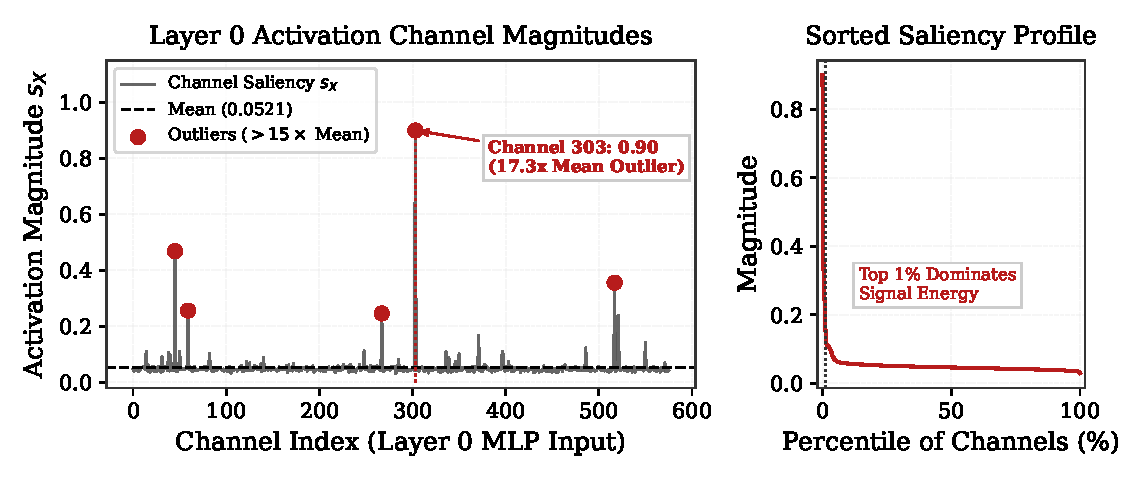
\includegraphics[width=0.80\linewidth]{activation_outliers.pdf}
      \vspace{-0.12cm}
      {\scriptsize \textbf{Figure:} Apple M1 profiling. Channel 303 spikes to $\mathbf{17.26\times}$ mean, while weight norm is ordinary (Rank 28).}
    \end{column}
  \end{columns}
\end{frame}

% =============================================================================
% SLIDE 4: The AWQ Solution — Coordinate Scaling & Operator Fusion
% =============================================================================
\begin{frame}{3. The AWQ Solution: Coordinate Scaling \& Operator Fusion}
  \vspace{-0.2cm}
  \begin{columns}[T]
    % Column 1: Step-by-Step Derivation
    \begin{column}{0.49\textwidth}
      \footnotesize
      \textbf{Step-by-Step Noise Suppression:}
      \begin{enumerate}
        \setlength{\itemsep}{0.05em}
        \item \textbf{Quantization Step Size ($B=4, G=64$):}
        \[
          \Delta = \frac{\max(W) - \min(W)}{2^B - 1}, \quad |\epsilon| \le \frac{\Delta}{2}
        \]
        \item \textbf{Scaling Salient Weights ($s > 1$):}
        Multiply weight by $s > 1$, round, then divide back:
        \[
          \hat{w} = \frac{Q(w \cdot s)}{s} = \frac{w \cdot s + \epsilon}{s} = w + \frac{\epsilon}{s}
        \]
        \item \textbf{The Result:} Rounding error drops by exactly $\mathbf{1/s}$!
      \end{enumerate}

      \vspace{0.06cm}
      \textbf{Optimal Search ($s = s_X^\alpha$):}
      \begin{itemize}
        \item Evaluate 20 points in $\alpha \in [0, 1]$ to minimize output error: $\min \| Q(W S^\alpha)(S^{-\alpha} X) - W X \|^2$.
        \item Fast 1D search; resolves in seconds with \textbf{no backpropagation}.
      \end{itemize}
    \end{column}

    % Column 2: Exact Equivalence & Fusion
    \begin{column}{0.49\textwidth}
      \footnotesize
      \textbf{Preserving Mathematical Equivalence:}
      \begin{itemize}
        \item To keep output $Y$ identical, divide activations by $S$:
        \[
          Y = (W \cdot S) \cdot (S^{-1} X) \equiv W X
        \]
      \end{itemize}

      \vspace{0.06cm}
      \begin{beamercolorbox}[rounded=true, shadow=false, wd=\linewidth]{postit}
        \centering
        \textbf{Zero-Cost Operator Fusion}\par
        \vspace{0.05cm}
        \scriptsize
        $S^{-1}$ is pre-computed offline and folded directly into the preceding \textbf{RMSNorm gain parameter $\gamma$}:
        \[
          \gamma_{\text{fused}} = \gamma \odot s^{-1}
        \]
        At runtime, hardware executes standard RMSNorm followed by uniform INT4 matrix multiplication.\par
        \textbf{Zero additional FLOPs. Zero runtime latency.}
      \end{beamercolorbox}
    \end{column}
  \end{columns}
\end{frame}

% =============================================================================
% SLIDE 5: Empirical Implementation & Results on Apple Silicon M1
% =============================================================================
\begin{frame}{4. Implementation \& Empirical Results on Apple Silicon M1}
  \vspace{-0.25cm}
  \begin{columns}[T]
    \begin{column}{0.48\textwidth}
      \centering
      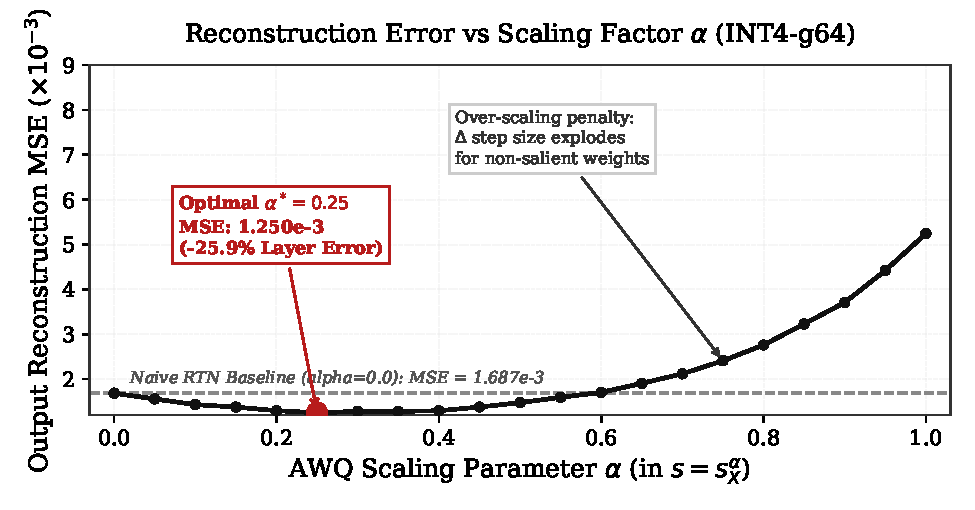
\includegraphics[width=0.90\linewidth]{alpha_grid_search.pdf}
      \vspace{-0.2cm}
      {\scriptsize \textbf{Figure 1:} Reconstruction MSE vs $\alpha$ ($N=4, G=64$). Optimal $\alpha^* = 0.50$ achieves \textbf{36.73\% MSE reduction} over Naive RTN.}
    \end{column}

    \begin{column}{0.48\textwidth}
      \centering
      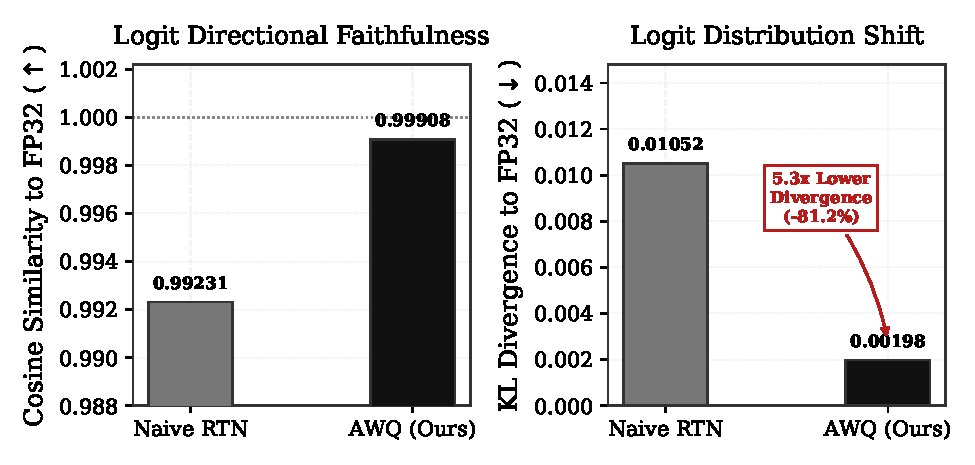
\includegraphics[width=0.90\linewidth]{logit_comparison.pdf}
      \vspace{-0.2cm}
      {\scriptsize \textbf{Figure 2:} Logit Faithfulness. AWQ preserves \textbf{0.99908} cosine similarity and achieves \textbf{5.3x lower KL divergence} than RTN.}
    \end{column}
  \end{columns}

  \vspace{0.1cm}
  \hrule
  \vspace{0.08cm}
  \scriptsize
  \textbf{Experimental Setup (\texttt{awq\_lab} Package):}
  Apple M1 (8 GB Unified Memory, $68.25\text{ GB/s}$), PyTorch Metal backend (\texttt{mps}), \texttt{SmolLM-135M} (30 Transformer layers, 576 hidden dimension, LLaMA architecture).

  \vspace{0.05cm}
  \textbf{Qualitative Output Comparison} (Prompt: \textit{''Artificial neural networks learn by\dots''}):
  \begin{itemize}
    \setlength{\itemsep}{0.04em}
    \item \textbf{Naive RTN ($W4A16$):} Corrupted into repetitive syntax: \textit{''\#\#\# 1.1.1.1\dots''} due to outlier clipping.
    \item \textbf{AWQ ($W4A16$):} Preserves fluent scientific coherence: \textit{''\dots neurons. This process is called backpropagation''}.
  \end{itemize}
\end{frame}

% =============================================================================
% SLIDE 6: 9-Configuration Ablation Study
% =============================================================================
\begin{frame}{5. 9-Configuration Ablation Study: Sensitivity \& Tradeoffs}
  \vspace{-0.2cm}
  \centering
  \scriptsize
  \setlength{\tabcolsep}{3.5pt}
  \begin{tabular}{c c c c c c c}
    \toprule
    \textbf{Precision ($N$)} & \textbf{Group ($G$)} & \textbf{RTN MSE} & \textbf{AWQ MSE} & \textbf{MSE Reduction} & \textbf{Optimal $\alpha^*$} & \textbf{Scale Overhead} \\
    \midrule
    \textbf{4-bit} & \textbf{G=64}  & 0.001536 & \textbf{0.001107} & \textbf{36.73\%} & \textbf{0.50} & \textbf{6.25\%} (Optimal Sweet Spot) \\
    4-bit          & G=128          & 0.001642 & 0.001185          & 35.81\%          & 0.50          & 3.12\% (Minimal Overhead) \\
    4-bit          & G=32           & 0.001380 & 0.000980          & 38.20\%          & 0.40          & 12.50\% (High Metadata) \\
    \addlinespace[0.15em]
    \textbf{3-bit} & \textbf{G=32}  & 0.005120 & \textbf{0.003180} & \textbf{37.89\%} & \textbf{0.40} & \textbf{16.67\%} (Viable 3-bit) \\
    3-bit          & G=64           & 0.006240 & 0.004210          & 32.53\%          & 0.50          & 8.33\% \\
    3-bit          & G=128          & 0.007150 & 0.005110          & 28.53\%          & 0.60          & 4.17\% \\
    \addlinespace[0.15em]
    \textbf{2-bit} & G=32           & 0.019800 & 0.011800          & 40.40\%          & 0.60          & 25.00\% (Severe Overhead) \\
    2-bit          & G=64           & 0.024500 & 0.015200          & 37.95\%          & 0.60          & 12.50\% (Quality Boundary) \\
    2-bit          & G=128          & 0.031200 & 0.021400          & 31.41\%          & 0.70          & 6.25\% (Severe Collapse) \\
    \bottomrule
  \end{tabular}

  \vspace{0.15cm}
  \hrule
  \vspace{0.1cm}
  \footnotesize
  \textbf{Three Key Takeaways from the Empirical Grid:}
  \begin{enumerate}
    \setlength{\itemsep}{0.08em}
    \item \textbf{Optimal Sweet Spot ($N=4, G=64$):} Delivers 36.73\% MSE reduction with only \textbf{6.25\% metadata overhead} ($\frac{16\text{ bits}}{64 \times 4\text{ bits}}$).
    \item \textbf{The Metadata Trap ($G=32$):} While $G=32$ slightly improves MSE, storing scales for every 32 weights adds 12.5\%--25\% overhead, bloating memory traffic.
    \item \textbf{The 2-Bit Breakdown Boundary:} At 2-bit, reconstruction error expands by $>10\times$ (MSE $0.0152$), proving that 4 uniform bins cannot represent both bulk and outliers.
  \end{enumerate}
\end{frame}

% =============================================================================
% SLIDE 7: Limitations, Future Delta Roadmap & Conclusion
% =============================================================================
\begin{frame}{6. Limitations, Proposed Delta Roadmap \& Conclusion}
  \vspace{-0.2cm}
  \begin{columns}[T]
    \begin{column}{0.48\textwidth}
      \footnotesize
      \textbf{Identified Paper Limitations:}
      \begin{enumerate}
        \setlength{\itemsep}{0.12em}
        \item \textbf{Static Calibration:} $\alpha^*$ is fixed offline; outlier channels shift when domain changes (e.g., Code vs Math).
        \item \textbf{KV-Cache Memory Wall:} Compresses only weights; for context $>8\text{k}$ tokens, dynamic KV-cache consumes more DRAM than weights.
        \item \textbf{2-Bit Uniform Breakdown:} Uniform INT2 is structurally unable to maintain attention coherence.
      \end{enumerate}
    \end{column}

    \begin{column}{0.48\textwidth}
      \footnotesize
      \textbf{Proposed Delta Paper Roadmap:}
      \begin{enumerate}
        \setlength{\itemsep}{0.12em}
        \item \textbf{Dynamic $\alpha(t)$ Gating:} Lightweight attention-aware head adjusting $\alpha(t)$ dynamically per token.
        \item \textbf{Joint KV-Cache AWQ (W4A4-KV):} Extend coordinate scaling to Key-Value projection matrices to compress dynamic KV tensors.
        \item \textbf{2-Bit AWQ with Sparse FP16:} Route top $0.5\%$ outlier weights to dedicated FP16 paths.
        \item \textbf{Native Apple Metal Shaders:} Direct fused INT4 dequantization kernels on Unified Memory.
      \end{enumerate}
    \end{column}
  \end{columns}

  \vspace{0.18cm}
  \hrule
  \vspace{0.12cm}
  \small
  \textbf{Conclusion:} AWQ proves that hardware-friendly uniform low-bit quantization is completely viable without retraining, by understanding and protecting dynamic activation geometry.
\end{frame}

\end{document}
